\chapter{Proverb 18}
\begin{figure}
  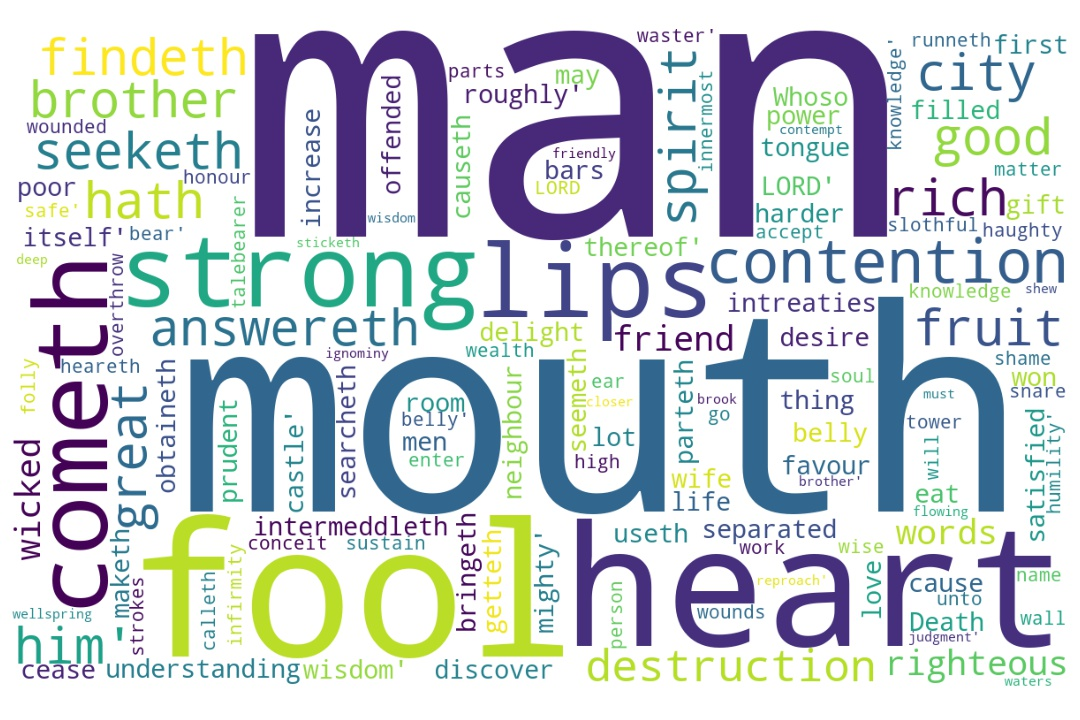
\includegraphics[width=\linewidth]{20OT-Proverbs/Proverb18-WordCloud.jpg}
  \caption{Proverb 18 Word Cloud}
  \label{fig:Proverb 18 word Cloud}
\end{figure}

\marginpar{\scriptsize \centering \fcolorbox{bone}{lime}{\textbf{A MAN FOCUSED ON GOD}}\\ (Proverbs 18:1-24) \begin{compactenum}[I.][8]
    \item Will be an \textbf{Inspired Man} - 
    \item Will be \textbf{Separate from the Ignorant Masses} - 
    \item For him most things in life will have  
    \textbf{Insignificant Meaning} - 
    \item Lives in an \textbf{Isolated Manner} 
    \item Lives by an \textbf{Individual Mandate} 
    \item Has an \textbf{intense and Insular Mentality}
\end{compactenum}}

\marginpar{\scriptsize \centering \fcolorbox{bone}{yellow}{\textbf{A FRIEND LIKE JESUS}}\\ (Proverb 18:24) \begin{compactenum}[I.][8]
    \item A \textbf{Close} Friend
    \item A \textbf{Constant} Friend
    \item A \textbf{Confiding} Friend
    \item A \textbf{Concerned} Friend
    \item A \textbf{Continuing} Friend
    \item A \textbf{Capable} Friend
    \item A \textbf{Caring} Friend
\end{compactenum}}

\marginpar{\scriptsize \centering \fcolorbox{bone}{black}{\textbf{\textcolor{white}{THE PURSUIT OF WISDOM}}}\\ (Proverb 18:24) \begin{compactenum}[I.][8]
    \item Then \textbf{Perverted} Motive -- to learn how manipulate events and circumstances. \index[scripture]{Proverbs!Pro 18:01}(Proverb 18:1)
    \item Then \textbf{Prideful} Motive -- To become exalted as wise. 
    \item Then \textbf{Public} Motive -- to be known and famous. 
    \item Then \textbf{Personal} Motive -- to achieve understanding. 
    \item Then \textbf{Practical} Motive -- to learn how live without mistakes or errors. 
    \item Then \textbf{Purposeful} Motive -- to learn navigate a specific problem. 
    \item Then \textbf{Perfect} Motive -- to learn how to live righteously before God. 
\end{compactenum}}

\marginpar{\scriptsize \centering \fcolorbox{bone}{blue}{\textbf{\textcolor{white}{WHAT YOUR SPEECH REVEALS}}}\\ (Proverb 18:4) \begin{compactenum}[I.][8]
    \item \textbf{Your Education} 
    \item \textbf{Your Excellence} 
    \item \textbf{Your Excitements} 
    \item \textbf{Your Enmity} 
    \item \textbf{Your Enemies} 
    \item \textbf{Your End} 
    \item \textbf{Your Emptiness}
    \item \textbf{Your Entanglements} 
\end{compactenum} }

\marginpar{\scriptsize \centering \fcolorbox{bone}{orange}{\textbf{THE WISE MAN}}\\ (Proverbs 18:1-24) \begin{compactenum}[I.][8]
    \item \textbf{Is Distinctive}
    \item \textbf{Is Disciplined}
    \item \textbf{Ignores Distractions}
    \item \textbf{Finds Delights in Wisdom}
    \item \textbf{Has Departed from the Common and Mundane}
    \item \textbf{Has a Distaste for Foolishness}
    \item \textbf{Is often regarded as Disturbed}
\end{compactenum} }




\footnote{\textcolor[cmyk]{0.99998,1,0,0}{\hyperlink{TOC}{Return to end of Table of Contents.}}}\footnote{\href{https://www.audioverse.org/english/audiobibles/books/ENGKJV/O/Prov/1}{\textcolor[cmyk]{0.99998,1,0,0}{Proverbs Audio}}}\textcolor[cmyk]{0.99998,1,0,0}{Through desire a man, having separated himself, seeketh \emph{and} \fcolorbox{bone}{MYGOLD}{intermeddleth} with all wisdom.}
[2] \textcolor[cmyk]{0.99998,1,0,0}{A fool hath no delight in \fcolorbox{bone}{MYGOLD}{understanding}, but that \fcolorbox{bone}{bone}{his} heart may discover itself.}
[3] \textcolor[cmyk]{0.99998,1,0,0}{When the wicked cometh, \emph{then} cometh also contempt, and with ignominy reproach.}
[4] \textcolor[cmyk]{0.99998,1,0,0}{The words of a man's mouth \emph{are} \emph{as} deep waters, \emph{and} the wellspring of wisdom \emph{as} a flowing brook.}\footnote{\textbf{Proverb 16:22} - Understanding is a wellspring of life unto him that hath it: but the instruction of fools is folly.}
[5] \textcolor[cmyk]{0.99998,1,0,0}{\emph{It} \emph{is} not good to accept the person of the wicked, to overthrow the righteous in judgment.}
[6] \textcolor[cmyk]{0.99998,1,0,0}{A fool's lips enter into contention, and \fcolorbox{bone}{bone}{his} mouth calleth for strokes.}
[7] \textcolor[cmyk]{0.99998,1,0,0}{A fool's mouth \emph{is} \fcolorbox{bone}{bone}{his} destruction, and \fcolorbox{bone}{bone}{his} lips \emph{are} the snare of \fcolorbox{bone}{bone}{his} soul.}
[8] \textcolor[cmyk]{0.99998,1,0,0}{The words of a talebearer \emph{are} as wounds, and they go down into the innermost parts of the belly.}
[9] \textcolor[cmyk]{0.99998,1,0,0}{He also that is slothful in \fcolorbox{bone}{bone}{his} work is brother to him that is a great waster.}
[10] \textcolor[cmyk]{0.99998,1,0,0}{The name of the LORD \emph{is} a strong tower: the righteous runneth into it, and is safe.}
[11] \textcolor[cmyk]{0.99998,1,0,0}{The rich man's wealth \emph{is} \fcolorbox{bone}{bone}{his} strong city, and as an high wall in \fcolorbox{bone}{bone}{his} own conceit.}
[12] \textcolor[cmyk]{0.99998,1,0,0}{Before destruction the heart of man is haughty, and before honour \emph{is} humility.}
[13] \textcolor[cmyk]{0.99998,1,0,0}{He that answereth a matter before he heareth \emph{it}, it \emph{is} folly and shame unto him.}
[14] \textcolor[cmyk]{0.99998,1,0,0}{The spirit of a man will sustain \fcolorbox{bone}{bone}{his} infirmity; but a wounded spirit who can bear?}
[15] \textcolor[cmyk]{0.99998,1,0,0}{The heart of the prudent getteth knowledge; and the ear of the wise seeketh knowledge.}
[16] \textcolor[cmyk]{0.99998,1,0,0}{A man's gift maketh room for him, and bringeth him before great men.}
[17] \textcolor[cmyk]{0.99998,1,0,0}{\emph{He} \emph{that} \emph{is} first in \fcolorbox{bone}{bone}{his} own cause \emph{seemeth} just; but \fcolorbox{bone}{bone}{his} neighbour cometh and searcheth him.}
[18] \textcolor[cmyk]{0.99998,1,0,0}{The lot causeth contentions to cease, and parteth between the mighty.}
[19] \textcolor[cmyk]{0.99998,1,0,0}{A brother offended \emph{is} \emph{harder} \emph{to} \emph{be} \emph{won} than a strong city: and \emph{their} contentions \emph{are} like the bars of a castle.}
[20] \textcolor[cmyk]{0.99998,1,0,0}{A man's belly shall be satisfied with the fruit of \fcolorbox{bone}{bone}{his} mouth; \emph{and} with the increase of \fcolorbox{bone}{bone}{his} lips shall he be filled.}
[21] \textcolor[cmyk]{0.99998,1,0,0}{Death and life \emph{are} in the power of the tongue: and they that love it shall eat the fruit thereof.}
[22] \textcolor[cmyk]{0.99998,1,0,0}{\emph{Whoso} findeth a wife findeth a good \emph{thing}, and obtaineth favour of the LORD.}
[23] \textcolor[cmyk]{0.99998,1,0,0}{The poor useth intreaties; but the rich answereth roughly.}
[24] \textcolor[cmyk]{0.99998,1,0,0}{A man \emph{that} \emph{hath} friends must shew himself friendly: and there is a friend \emph{that} sticketh closer than a brother.}


